% sh /Users/morril01/Documents/PhD/CDA_in_Cancer/text/other_presentations/FirstYearViva/compile.sh

%  You will then be invited to give a PowerPoint presentation outlining progress and future plans, with your ideas for input and advice from the committee

\documentclass{beamer}
\usepackage{color}
\usepackage{array}
\usepackage{tcolorbox}
\usepackage{tikz}
\usepackage{dsfont}
\usetikzlibrary{shapes.gates.logic.US,trees,positioning,arrows}
\usepackage[backend=bibtex, maxnames=10000]{biblatex}
\usepackage{calc}% for basic arithmetic
\usepackage{color, colortbl}
%\definecolor{LightCyan}{rgb}{0.88,1,1}
%\definecolor{LightCyan}{RGB}{234,234,236}
\definecolor{LightCyan}{RGB}{28,57,187}
\usepackage[first=0,last=9]{lcg}
\newcommand{\ra}{\rand0.\arabic{rand}}

%\setbeamercolor{palette primary}{bg=LightCyan,fg=white}
%\setbeamercolor{palette secondary}{bg=LightCyan,fg=white}
%\setbeamercolor{palette tertiary}{bg=LightCyan,fg=white}
%\setbeamercolor{palette quaternary}{bg=LightCyan,fg=white}
%\setbeamercolor{structure}{fg=LightCyan} % itemize, enumerate, etc
%\setbeamercolor{section in toc}{fg=LightCyan} % TOC sections


\bibliography{../../progress_text/bibliography.bib}
\renewcommand*{\bibfont}{\scriptsize}
\setbeamertemplate{bibliography item}{\insertbiblabel}

\newcommand{\mcrot}[4]{\multicolumn{#1}{#2}{\rlap{\rotatebox{#3}{#4}~}}} 

\newcommand*{\twoelementtable}[3][l]%
{%  
    \renewcommand{\arraystretch}{0.8}%
    \begin{tabular}[t]{@{}#1@{}}%
        #2\tabularnewline
        #3%
    \end{tabular}%
}

\mode<presentation>
{
  \usetheme{Warsaw}
%  \usefonttheme{structureitalicserif}
} 


\newcolumntype{L}[1]{>{\raggedright\let\newline\\\arraybackslash\hspace{0pt}}m{#1}}
\newcolumntype{C}[1]{>{\centering\let\newline\\\arraybackslash\hspace{0pt}}m{#1}}
\newcolumntype{R}[1]{>{\raggedleft\let\newline\\\arraybackslash\hspace{0pt}}m{#1}}

    \setbeamertemplate{headline}{}





\begin{document}


\begin{frame}{Signatures for CN: how do embed CN in matrix form}

\begin{itemize}
\item Each sample contains several features (independent of each other), each feature can be categorised into multiple components
	\begin{itemize}
	\item Geoff's signatures: features are concatenated
	\item \href{https://epubs.siam.org/doi/abs/10.1137/1.9781611972832.28?mobileUi=0}{*Multi-View Clustering via Joint Nonnegative Matrix Factorization*}
	\end{itemize}
\item Each sample contains many segments, each segment has multiple characteristics which can be categorised as compartments of features (Shiraishi)
	\begin{itemize}
	\item Equivalent to SNV, but for multiple features (instead of the single trinucleotide change)
	\item You can potentially get inspired by \href{https://www.biorxiv.org/content/10.1101/2021.05.16.444385v1}{*Mutational signatures of complex genomic rearrangements in human cancer*}
	\end{itemize}
\end{itemize}

\end{frame}

\begin{frame}{To do (?)}
\begin{enumerate}
\item Run Geoff's signature extraction, Shiraishi's minimal example
\item For Shiraishi's method: define segment-specific features, and categorise each feature in each segment to get the input matrix for pmsignature
\item Create github repo if you think it'd be useful
\end{enumerate}
\end{frame}

\begin{frame}{To do (?)}
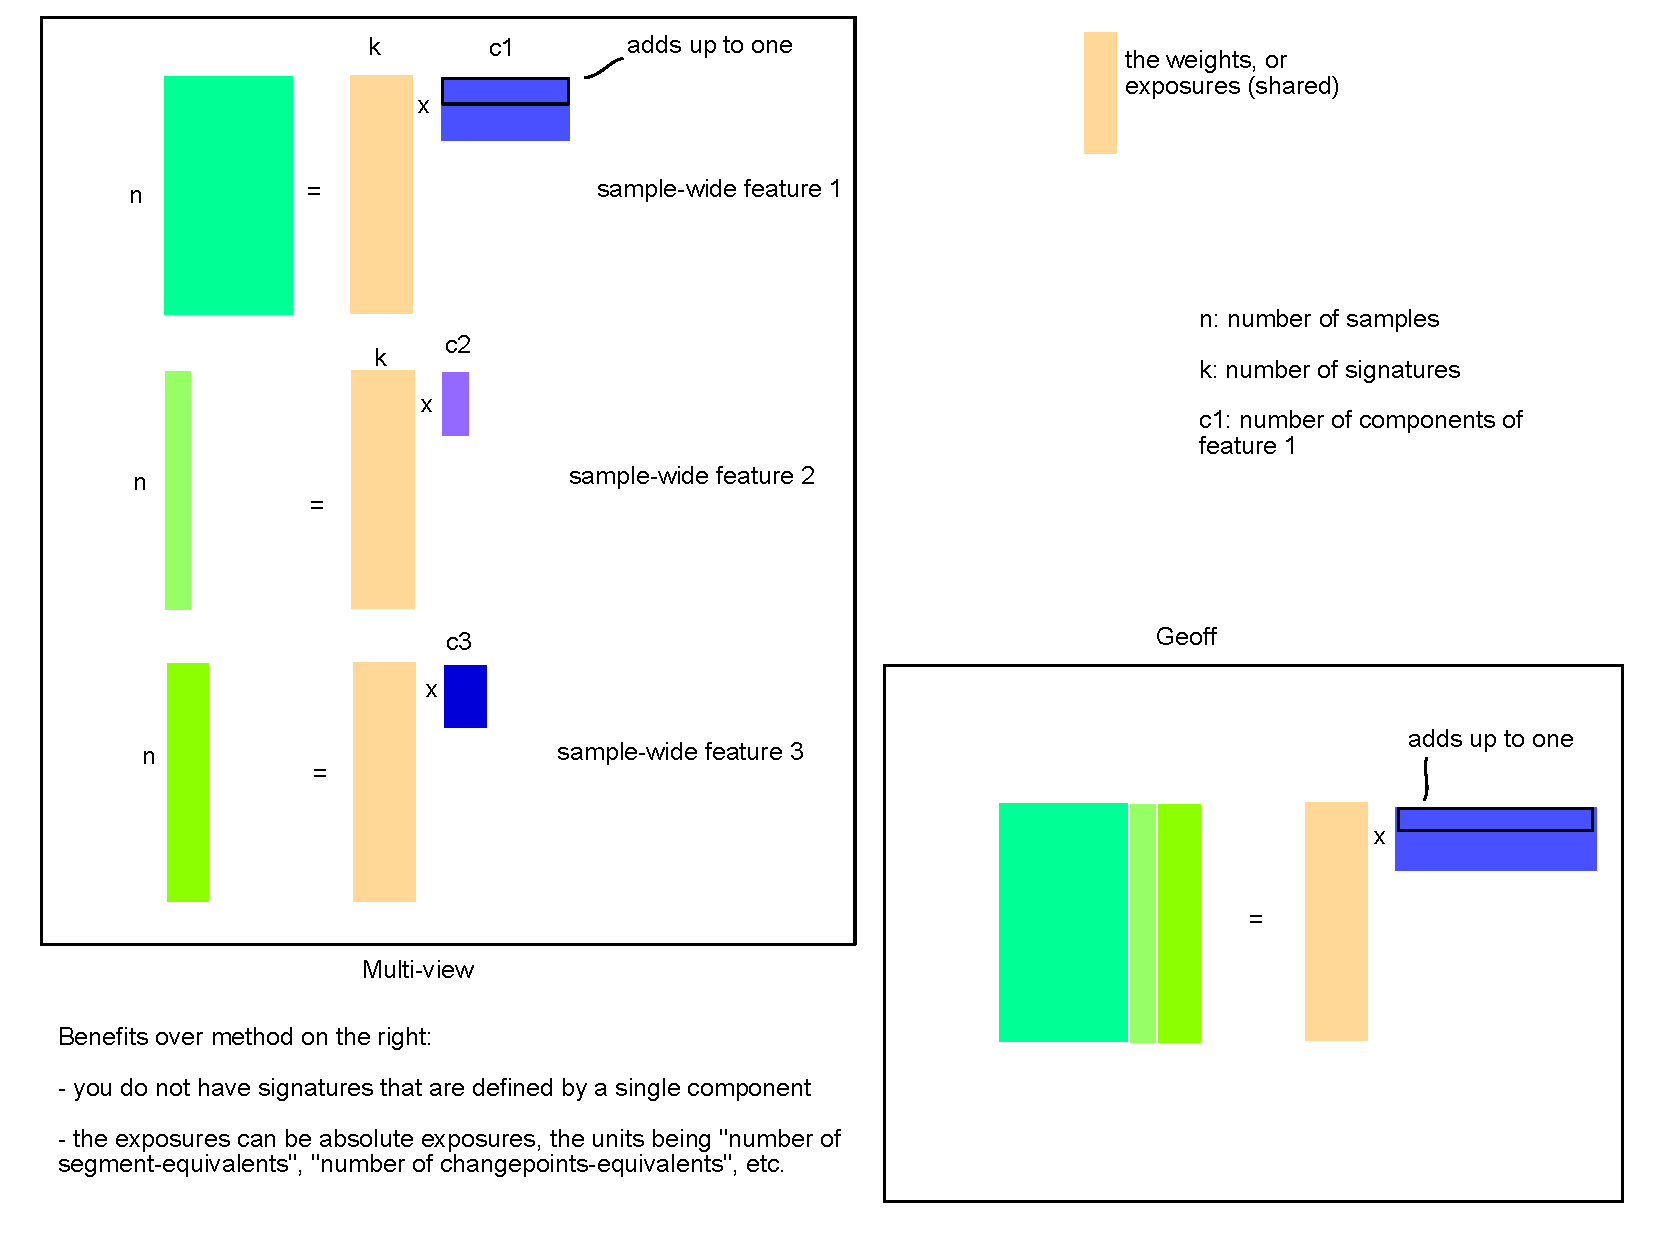
\includegraphics[width=\textwidth]{../../figures/joint_nmf}

\end{frame}

\end{document}
